\documentclass{article}
\usepackage{tikz}
\usetikzlibrary{arrows, positioning, automata}
\begin{document}

\begin{figure}
	\centering
	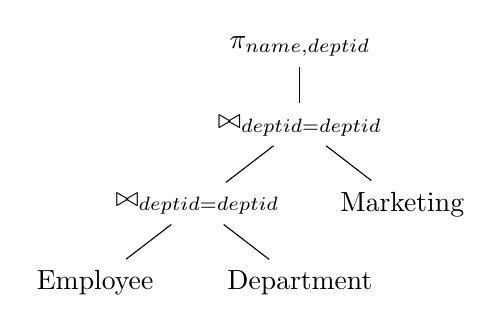
\begin{tikzpicture}[>=stealth',shorten >=1pt, node distance=1cm, on grid, initial/.style={}]

		\node[rectangle] (T0) 																			{$\pi_{name,deptid}$};
		\node[rectangle] (T1) 	[below =of T0] 											{$\bowtie_{deptid=deptid}$};
		\node[rectangle] (T2a) 	[below left=1cm and 1.3cm of T1] 		{$\bowtie_{deptid=deptid}$};
		\node[rectangle] (T3a)	[below right=1cm and 1.3cm of T2a] 	{Department};
		\node[rectangle] (T3b)	[below left=1cm and 1.3cm of T2a] 	{Employee};

		\node[rectangle] (T2b) [below right=1cm and 1.3cm of T1] 		{Marketing};
		
    \path (T0) edge (T1);
    \path (T1) edge (T2a);
    \path (T1) edge (T2b);
    \path (T2a) edge (T3a);
    \path (T2a) edge (T3b);

	\end{tikzpicture}
	\caption{The query tree}
\end{figure}

\end{document}
